\section{Microservice Architecture}

\begin{frame}{Microservice Architecture}
    \begin{itemize}
        \item Bisher: SOA - Aufteilung in Services
        \item Jetzt: feiner granulierte und vollständig isolierte Services
        \item Jeder Service hat eigene private Persistenz
        \item Kommunikation untereinander über Netzwerkprotokolle
        \item API-Gateway vermittelt zwischen Client und Services
    \end{itemize}
\end{frame}

\begin{frame}{Microservice Architecture: Struktur}
    \begin{figure}[!h]
        \centering
        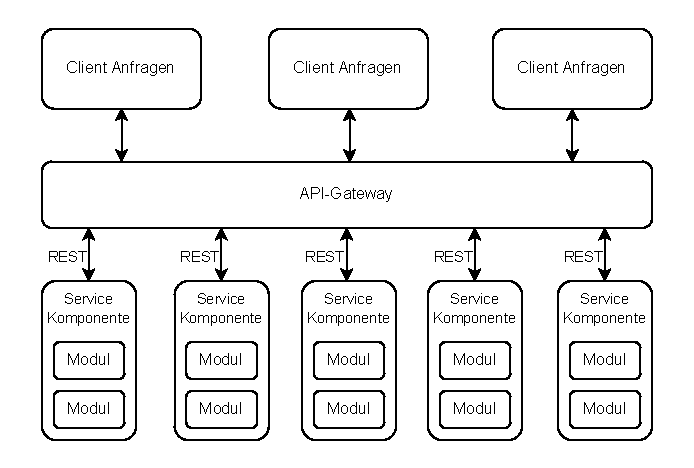
\includegraphics[scale=0.6]{imglib/microservices/microservices}
        \caption{Aufbau einer Microservices Architecture}
        \label{fig:microservices}
    \end{figure}
\end{frame}

\begin{frame}{Microservice Architecture: Beispiel E-Commerce I}
    \begin{itemize}
        \item API-Gateway für Client Anfragen
        \item Auslagerung der Business Logik in isolierte Services
        \item Unabhängige Services für Bestellung, Bezahlung und Versand
        \item Aufteilung der zentralen Datenbank in private Persistenzen
        \item Erweiterung durch zusätzliche Services, horizontale Skalierung gut möglich
        \item Architekturmuster sehr passend für Anwendungsfall
    \end{itemize}
\end{frame}

\begin{frame}{Microservice Architecture: Beispiel E-Commerce II}
    \begin{figure}[!h]
        \centering
        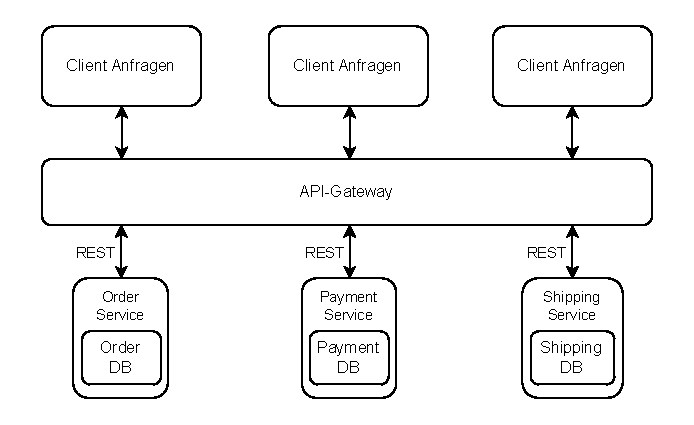
\includegraphics[scale=0.6]{imglib/microservices/ecommerce-microservices}
        \caption{E-Commerce-Beispiel mit Microservices Architecture}
        \label{fig:microservices-ecommerce}
    \end{figure}
\end{frame}

\begin{frame}{Microservice Architecture: Agilität}
    \begin{itemize}
        \item Lose Kopplung der Services $\Rightarrow$ einfaches Testen, Ausliefern und Entwickeln
        \item Kürzere Iterationen durch einfache Regressionstests
        \item Live-Deployments können ohne Downtime aktualisiert werden
        \item Services separat voneinander skalierbar
        \item Aber: Geringere Performance als andere Muster, da Netzwerklatenzen
        \item Aber: Aufwendige Integrationstests durch hohe Anzahl an Komponenten
        \item Aber: Initialer Aufwand höher, da Spezifizierung von Schnittstellen und Architektur nötig~\cite{architecturePatterns}
        \item Fazit: In vielen agilen Umgebungen sinnvoll, aber angemessene Granularität und korrekte Aufteilung wichtig
    \end{itemize}
\end{frame}
